\renewcommand{\thefigure}{A\arabic{figure}}
\setcounter{figure}{0}   

\section{Model}
\subsection{Notation}
Before presenting the model we describe some notation used through out the appendix. For a $m \times n$ matrix $r$ we use the following broadcasting notation $\mv{r}_{k,j:l}=[ r_{k,j}, r_{k,j+1}, \ldots, r_{k,l}]$.
Further $x | y \sim \pi(.)$ implies that the random variable $x$ if we conditioning on $y$ follows distribution $\pi(.)$.
The relevant variables in the model are the following:

	\begin{tabularx}{\linewidth}{ccL}
		Variable name & Dimension & Description \\  \hline
		$\mv{d}$ & $T \times 1$ & $d_i$ is the number of deaths that occurred day $i$. \\
		$\mv{r}$ & $T \times T$ & $r_{ij}$ is number of death recorded for day $i$ at day $j$.  Note that $r_{ij}$ for $i<j$ is not defined.   \\
		$\mv{p}$ & $T \times T$ & $p_{ij}$ is the probability of that a death for day $i$ not yet recorded is recorded at day $j$.
		  Note that $p_{ij}$ for $i<j$ is not defined.  \\
		$\mv{\alpha}$ & $K \times 1$ & Latent prior parameter for $\mv{p}$ \\
		$\mv{\beta}$ & $K \times 1$ & Latent prior parameter for $\mv{p}$ \\
		$\mv{\alpha}^H$ & $2 \times 1$ & parameter for the probability, $\mv{p}$ for holiday adjustment. \\
		$\mv{\beta}^H$ & $2 \times 1$ & parameter for the probability, $\mv{p}$ for holiday adjustment. \\
		$\mv{\mu}$ &  $T \times 1$ &  $\mu_i$  is the intensity of the expected number of deaths at day $i$. \\
		$\sigma^2$ & $1\times 1$ & Variation of the random walk prior for the log intensity. \\
		$\phi$ & $1\times 1$ & overdispersion parameter for negative binomial distribution. \\
		$p_0$ & $1\times 1$ & probability of reporting for a low reporting event. \\
		$pi$ & $1\times 1$ & probability of a low reporting event.
	\end{tabularx}
\subsection{likelihood}
The most complex part of our model is the likelihood, i.e. the density of the observations given the parameters. Here the data consist the daily report of recorded deaths for the past days. This can conveniently be represented upper triangular matrix, $\mv{r}$, where $r_{i,j}$ represents number of new reported deaths for day $i$ reported at day $j$. This matrix is displayed on the left in Table \ref{tab:Data}.

\begin{table}
	\centering
	\begin{tabular}{cccccc}
		\multicolumn{1}{c}{} & \multicolumn{5}{c}{Reported date}                                             \\
		\parbox[t]{2mm}{\multirow{5}{*}{\rotatebox[origin=c]{90}{Death date}}}   & $r_{11}$ & $r_{12}$ & $\cdots$ &$\cdots$  &  $r_{1T}$\\
		& & $r_{22}$ &  $\cdots$ & $\cdots$   &$r_{2T}$ \\
		& & &$r_{33}$ &  $\cdots$ &  $r_{3T}$ \\
		& & & &  $\ddots$ & $\vdots$  \\
		& & & &  &  $r_{TT}$ \\

	\end{tabular}

	\caption{The table describes the observations data.}
	\label{tab:Data}
\end{table}

 We assume that given the true number of deaths at day $i$, $d_i$, that each reported day $j$ the remaining death $d_i - \sum_{k=1}^{j-1}r_{i,k}$ each recored with probability $p_{ij}$, i.e. $$r_{i,j}|D_i,r_{1,1:j}.p \sim Bin(d_i - \sum_{k=1}^{j-1}r_{i,k}, p_{i,j}).$$

Typically in removal sampling one would set the probability of reporting uniform, i.e. $p_{i,j}:=p$. However for this data this is clearly not realistic given weekly patterns in reporting --very little reporting during the weekends. Instead we assume that we have $k$ different probabilities. Further, to account for overdispertion, we assume that each probability rather being a fixed scalar is a random variable with a Beta distribution. The Beta distribution has two parameters $\alpha$ and $\beta$. This resulting the following distribution for the probabilities
$$
p_{i,j}| \mv{\alpha},\mv{\beta}, \mv{\alpha}^H,\mv{\beta}^H  \sim Beta(\alpha^H_j\alpha_{min(j-i,k)},\beta^H_j\beta_{min(j-i,k)}).
$$
Here, if $j\in H$ then day $j$ is a holidays or weekends, and the parameters above are
$$
\alpha^H_j = \begin{cases}
\alpha_1^H \alpha_2^H & \mbox{if }  \{j\in H \}\cup  \{j-1\in H \},  \\
\alpha_1^H & \mbox{if }  \{j\in H \}\cup  \{j-1\in H^c \}, \\
\alpha_2^H & \mbox{if }  \{j\in H^c \}\cup  \{j-1\in H \}, \\
1 & \mbox{else,}
\end{cases}
$$
and
$$
\beta^H_j = \begin{cases}
\beta_1^H \beta_2^H & \mbox{if }  \{j\in H \}\cup  \{j-1\in H \},  \\
\beta_1^H & \mbox{if }  \{j\in H \}\cup  \{j-1\in H^c \}, \\
\beta_2^H & \mbox{if }  \{j\in H^c \}\cup  \{j-1\in H \}, \\
1 & \mbox{else.}
\end{cases}
$$
These extra parameters are created to account for the under-reporting that occurs during weekend and holidays.
Finally we add an extra mixture component that allows for very low reporting.

\subsection{Priors}
For the $\mv{\alpha}$ and $\mv{\beta}$ parameters we use an (improper) uniform prior. For the deaths, $\mv{d}$, one could imagine several different prior ideally some sort of epidemiological model. However, here we just assume a log-Gaussian Cox processes \citep{Moller1998_log_gaussian}, but instead of Poisson distribution we use a negative binomial to handle possible over dispersion. The latent Gaussian processes has a intrinsic random walk distribution \citep{Rue2005_gaussian_markov} i.e.
\begin{align*}
\log(\mu_i) - \log(\mu_{i-1}) &\sim N(0,\sigma^2),\\
d_i| \phi, \mu_i  &\sim NegBin(\mu_i, \phi).
\end{align*}
This model is created to create a temporal smoothing between the reported deaths.
For the hyperparameter $\sigma^2$ we impose a inverse Gamma distribution, this prior is suitable here because it guarantees that the process is not constant ($\sigma^2=0$) which we know is not the case.
\subsection{Full model}
Putting the likelihood and priors together we get the following hierarchical Bayesian model
\begin{align*}
\sigma^2 &\sim \Gamma(1,0.01) \\
\phi &\sim \Gamma(1,0.01) \\
\alpha_k &\sim U[0,\infty] \\
\beta_k &\sim U[0,\infty] \\
\alpha_k^H &\sim U[0,\infty] \\
\beta_k^H &\sim U[0,\infty] \\
\log(\mu_i) - \log(\mu_{i-1}) &\sim N(0,\sigma^2)\\
d_i| \phi,\mu_i  &\sim NegBin(\mu_i,\phi) \\
p_{i,j}|  \mv{\alpha},\mv{\beta}, \mv{\alpha}^H,\mv{\beta}^H &\sim Beta(\alpha^H_j\alpha_{min(j-i,k)},\beta^H_j\beta_{min(j-i,k)}) \\
r_{i,j}|d_i,\mv{r}_{1,1:j},p &\sim \pi Bin(d_i - \sum_{k=1}^{j-1}r_{i,k},p_0)+ (1-\pi) Bin(d_i - \sum_{k=1}^{j-1}r_{i,k}, p_{i,j}),
\end{align*}
where where and $j\leq i$ and $i=1,\ldots,T$.

\section{Inference}
As the main goal to generate inference of the number of death $\mv{d}$ is through the posterior distribution of number of deaths $\mv{d}$ given the observations $\mv{r}$.
In order to generate samples from this distribution we use a Markov Chain Monte Carlo method \citep{Brooks2011_handbook_markov}. In more detail we use a blocked Gibbs sampler, which generates samples in the following sequence:
\begin{itemize}
	\item  We sample $\mv{\alpha},\mv{\beta}, \mv{\alpha}^H,\mv{\beta}^H|\mv{d}, \mv{r}$ using the fact that one can integrate out $p$ in the model, and then  $\mv{d}|\mv{\alpha},\mv{\beta}, \mv{\alpha}^H,\mv{\beta}^H,\mv{r},\mv{\mu},\phi$  follows a Beta-Binomial distribution. Here to we use an adaptive MALA \citep{Atchade2006_adaptive_version} to sample from these parameters.
	\item  To sample $\mv{d}|\mv{\alpha},\mv{\beta}, \mv{\alpha}^H,\mv{\beta}^H,\mv{r},\mv{\mu},\phi$, that each death, $d_i$ is conditionally independent, and we just use a Metropolis Hastings random walk to sample each one.
	\item To sample $\mv{\mu} | \mv{d},\sigma^2,\phi$ we again use an adaptive MALA.
	\item Finally We sample $\sigma^2|\mv{d}$,and  $p_0,\pi$ directly since this distribution is explicit, and $\phi$ using a MH-RW.
\end{itemize}

\section{Model Benchmark}
In this section, we present additional comparison of the model to the benchmark. We first describe the benchmark model in detail.

The benchmark model simply takes the sum of average historical reporting lags for the preceding 14 days. As before $r_{ij}$ is the number of deaths that happened on day $i$ and were recorded on day $j$. To predict the number of people that died on a given day, we first calculate lag averages:

\begin{align}
    \hat{r}_{i, i+L} = \frac{\sum^{14}_{k=i-14} r_{k - L, k}}{14},
\end{align}

where $\hat{r}_{i, i+L}$ is the average number of deaths reported with a lag of $L$ days, based on the 14 reports closest preceding day $i$. If we are looking at data released $2020-04-28$ and call this day 0, the latest death date that we have 10-day ($L=10$) reporting lag observation for is $r_{-10,0}$. The average for $Lag(0, 10)$ is therefore taken over the 14 days between $r_{-24,-14}$ and $r_{-10,0}$ (2020-04-04 and 2020-04-18). For this reason, some of the earlier predictions will not have data from $14$ days. The average is then taken over all available reports.

In the comparisons we aim at predicting the total number of deaths that will have been reported within 14 days of the death date. To do so, we sum over the average lag that has yet to be reported. If we are predicting the number of people that have yet to be reported dead for day -3, we already know the true values for $r_{-3,-3}$, $r_{-3,-2}$, $r_{-3,-1}$, and $r_{-3,0}$ so we only need to predict $r_{-3,1}\ldots r_{-3,10}$. The prediction is then

\begin{align}
    Benchmark(i, j) = \sum_{l=i}^{j} r_{i,l}+ \sum_{l = j}^{14} \hat{r}_{i, l}.
\end{align}

As confidence interval we simply use a Normal assumption with standard deviations of the reporting lags, assuming independence, i.e. this is just the square root of the sum of $Var(\hat{r})$.

\begin{figure}
    \centering
    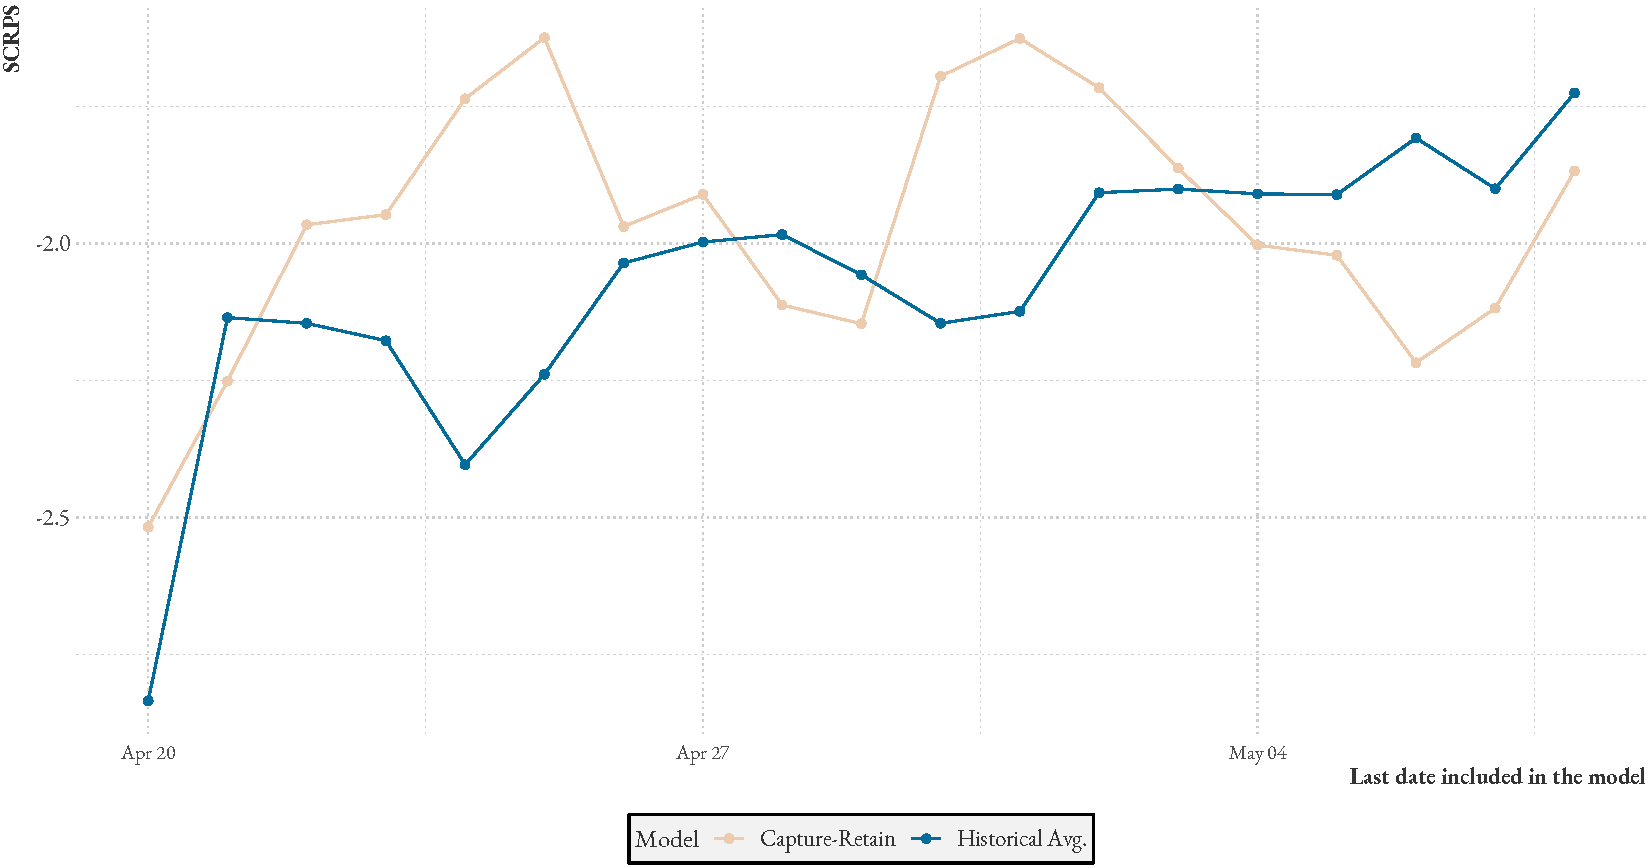
\includegraphics[width=0.9\textwidth]{../plots/SCRPS_over_states}
    \caption{Average SCRPS as the pandemic progresses.w}
    \label{fig:SCRPS_states}
\end{figure}

\begin{figure}
    \centering
    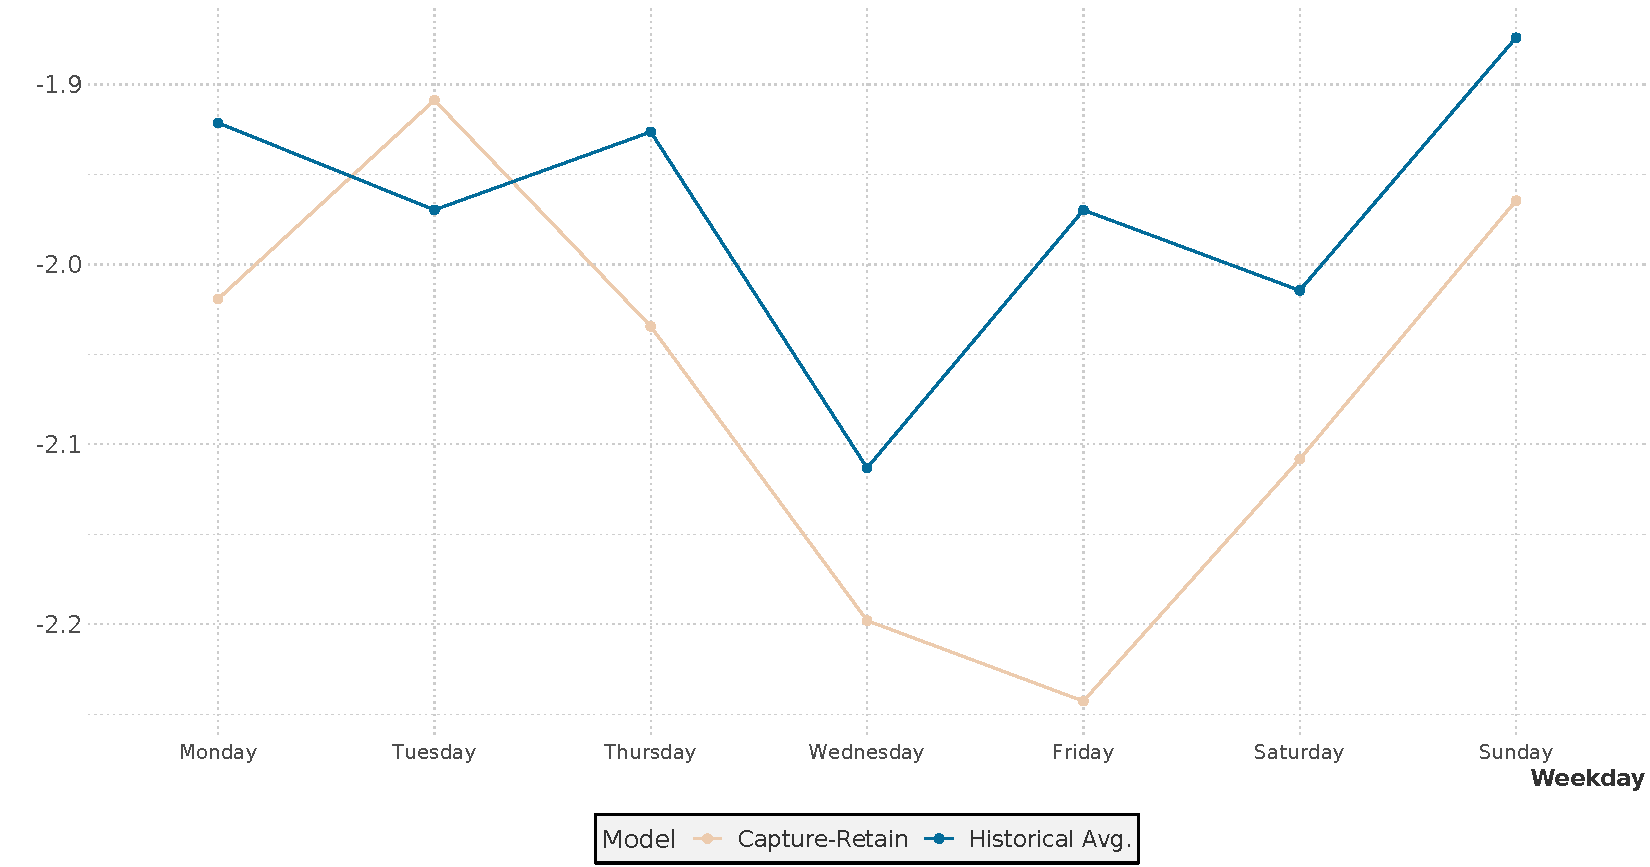
\includegraphics[width=0.9\textwidth]{../plots/SCRPS_over_weekdays}
    \caption{Average SCRPS per weekday.}
    \label{fig:SCRPS_weekdays}
\end{figure}